\documentclass[aspectratio=169]{beamer}
\usetheme{simple}

\RequirePackage[l2tabu, orthodox]{nag}


% \usepackage[left=1.in, right=1.in, top=1.25in, bottom=1.25in]{geometry}

% FONTS
%\usepackage[T1]{fontenc}

% Replace default Latin Modern typewriter with its proportional counterpart
% http://www.tug.dk/FontCatalogue/lmoderntypewriterprop/
%\renewcommand*\ttdefault{lmvtt}


%%% OPTION 1 - Fourier Math + New Century Schoolbook + ParaType Sans

% % Import Fourier Math (this imposes its own New Century Schoolbook type)
% % http://www.ctan.org/tex-archive/fonts/fouriernc/
%\usepackage{fouriernc}
%\usepackage{amsmath}
% % Replace with TeX Gyre Schola version of New Century Schoolbook (must scale!)
% % http://www.tug.dk/FontCatalogue/tgschola/
%\usepackage[scale=0.92]{tgschola}
%\usepackage[scaled=0.88]{PTSans}

%% OPTION 2 - MathDesign Math + Bitstream Charter + ParaType Sans

% Import MathDesign (this brings along Bitstream Charter)
% http://www.ctan.org/tex-archive/fonts/mathdesign/
\usepackage[bitstream-charter]{mathdesign}
\usepackage{amsmath}
\usepackage[scaled=0.92]{PTSans}


% %%% OPTION 3 - MTPRO 2 Math + Termes Times + ParaType Sans

% \usepackage{tgtermes}
% \usepackage{amsmath}
% \usepackage[subscriptcorrection,
%             amssymbols,
%             mtpbb,
%             mtpcal,
%             nofontinfo  % suppresses all warnings
%            ]{mtpro2}
% \usepackage{scalefnt,letltxmacro}
% \LetLtxMacro{\oldtextsc}{\textsc}
% \renewcommand{\textsc}[1]{\oldtextsc{\scalefont{1.10}#1}}
% \usepackage[scaled=0.92]{PTSans}

% Use default fonts here
\usepackage{amsmath}
\usepackage{amssymb}

% \usepackage{titling}

% % COLOR
% \usepackage[table,usenames,dvipsnames]{xcolor}
\definecolor{shadecolor}{gray}{0.9}

% SPACING and TEXT
\usepackage[final,expansion=alltext]{microtype}
\usepackage[english]{babel}
\usepackage[parfill]{parskip}
\usepackage{afterpage}
\usepackage{framed}
\usepackage{verbatim}
\usepackage{setspace}

\newenvironment{exercise}[1]
{
    \itshape
    \paragraph{Exercise: \textit{#1}}
}
{ 
}


% \usepackage[bottom]{footmisc}
\usepackage[symbol]{footmisc}
\renewcommand{\thefootnote}{\arabic{footnote}}


% FIGURES
\usepackage{graphicx}
\usepackage[labelfont={it, small}, 
            textfont={small,singlespacing},
            % justification={justified,RaggedRight},
            singlelinecheck=false,
            margin=0pt]{caption}
\usepackage[format=hang]{subcaption}
% \usepackage{ccaption}

% % APPENDIX FIGURES
% \usepackage{chngcntr}

% % TABLES
% \usepackage{booktabs}
% \usepackage{longtable}
% \usepackage{hhline}

% ALGORITHMS
\usepackage[algoruled]{algorithm2e}
\usepackage{listings}
\usepackage{fancyvrb}
\fvset{fontsize=\normalsize}

% % THEOREMS
\usepackage{amsthm}
\newtheorem{proposition}{Proposition}
% \newtheorem{lemma}{Lemma}

% % BIBLIOGRAPHY
\usepackage{natbib}

% HYPERREF
% \usepackage[colorlinks,linktoc=all]{hyperref}
% \usepackage[all]{hypcap}
% \hypersetup{citecolor=MidnightBlue}
% \hypersetup{linkcolor=black}
% \hypersetup{urlcolor=MidnightBlue}

% % CLEVEREF must come after HYPERREF
% \usepackage[nameinlink]{cleveref}

% % ACRONYMS
% \usepackage[acronym,smallcaps,nowarn]{glossaries}
% % \makeglossaries

% % COLOR DEFINITIONS
\newcommand{\red}[1]{\textcolor{BrickRed}{#1}}
\newcommand{\orange}[1]{\textcolor{BurntOrange}{#1}}
\newcommand{\green}[1]{\textcolor{OliveGreen}{#1}}
\newcommand{\blue}[1]{\textcolor{MidnightBlue}{#1}}
\newcommand{\gray}[1]{\textcolor{black!60}{#1}}

% LISTINGS DEFINTIONS
\lstdefinestyle{mystyle}{
    commentstyle=\color{OliveGreen},
    keywordstyle=\color{BurntOrange},
    numberstyle=\tiny\color{black!60},
    stringstyle=\color{MidnightBlue},
    basicstyle=\ttfamily,
    breakatwhitespace=false,
    breaklines=true,
    captionpos=b,
    keepspaces=true,
    numbers=left,
    numbersep=5pt,
    showspaces=false,
    showstringspaces=false,
    showtabs=false,
    tabsize=2
}
\lstset{style=mystyle}

\usepackage[colorinlistoftodos,
            prependcaption,
            textsize=small,
            backgroundcolor=yellow,
            linecolor=lightgray,
            bordercolor=lightgray]{todonotes}

\usepackage{soul}

\usepackage{media9}
% !TEX root = template.tex

% \DeclareRobustCommand{\mb}[1]{\ensuremath{\boldsymbol{\mathbf{#1}}}}
\DeclareRobustCommand{\mb}[1]{\boldsymbol{#1}}

% \newcommand{\KL}[2]{\ensuremath{\textrm{KL}\PARENS{#1\;\|\;#2}}}
\DeclareRobustCommand{\KL}[2]{\ensuremath{D_{\textrm{KL}}\left(#1\;\|\;#2\right)}}

\DeclareMathOperator*{\argmax}{arg\,max}
\DeclareMathOperator*{\argmin}{arg\,min}

\renewcommand{\mid}{~\vert~}
\newcommand{\given}{\,|\,}
\newcommand{\iid}[1]{\stackrel{\text{iid}}{#1}}

\newcommand{\mba}{\mb{a}}
\newcommand{\mbb}{\mb{b}}
\newcommand{\mbc}{\mb{c}}
\newcommand{\mbd}{\mb{d}}
\newcommand{\mbe}{\mb{e}}
% \newcommand{\mbbf}{\mb{f}}
\newcommand{\mbg}{\mb{g}}
\newcommand{\mbh}{\mb{h}}
\newcommand{\mbi}{\mb{i}}
\newcommand{\mbj}{\mb{j}}
\newcommand{\mbk}{\mb{k}}
\newcommand{\mbl}{\mb{l}}
\newcommand{\mbm}{\mb{m}}
\newcommand{\mbn}{\mb{n}}
\newcommand{\mbo}{\mb{o}}
\newcommand{\mbp}{\mb{p}}
\newcommand{\mbq}{\mb{q}}
\newcommand{\mbr}{\mb{r}}
\newcommand{\mbs}{\mb{s}}
\newcommand{\mbt}{\mb{t}}
\newcommand{\mbu}{\mb{u}}
\newcommand{\mbv}{\mb{v}}
\newcommand{\mbw}{\mb{w}}
\newcommand{\mbx}{\mb{x}}
\newcommand{\mby}{\mb{y}}
\newcommand{\mbz}{\mb{z}}

\newcommand{\mbA}{\mb{A}}
\newcommand{\mbB}{\mb{B}}
\newcommand{\mbC}{\mb{C}}
\newcommand{\mbD}{\mb{D}}
\newcommand{\mbE}{\mb{E}}
\newcommand{\mbF}{\mb{F}}
\newcommand{\mbG}{\mb{G}}
\newcommand{\mbH}{\mb{H}}
\newcommand{\mbI}{\mb{I}}
\newcommand{\mbJ}{\mb{J}}
\newcommand{\mbK}{\mb{K}}
\newcommand{\mbL}{\mb{L}}
\newcommand{\mbM}{\mb{M}}
\newcommand{\mbN}{\mb{N}}
\newcommand{\mbO}{\mb{O}}
\newcommand{\mbP}{\mb{P}}
\newcommand{\mbQ}{\mb{Q}}
\newcommand{\mbR}{\mb{R}}
\newcommand{\mbS}{\mb{S}}
\newcommand{\mbT}{\mb{T}}
\newcommand{\mbU}{\mb{U}}
\newcommand{\mbV}{\mb{V}}
\newcommand{\mbW}{\mb{W}}
\newcommand{\mbX}{\mb{X}}
\newcommand{\mbY}{\mb{Y}}
\newcommand{\mbZ}{\mb{Z}}

\newcommand{\mbalpha}{\mb{\alpha}}
\newcommand{\mbbeta}{\mb{\beta}}
\newcommand{\mbdelta}{\mb{\delta}}
\newcommand{\mbepsilon}{\mb{\epsilon}}
\newcommand{\mbchi}{\mb{\chi}}
\newcommand{\mbeta}{\mb{\eta}}
\newcommand{\mbgamma}{\mb{\gamma}}
\newcommand{\mbiota}{\mb{\iota}}
\newcommand{\mbkappa}{\mb{\kappa}}
\newcommand{\mblambda}{\mb{\lambda}}
\newcommand{\mbmu}{\mb{\mu}}
\newcommand{\mbnu}{\mb{\nu}}
\newcommand{\mbomega}{\mb{\omega}}
\newcommand{\mbphi}{\mb{\phi}}
\newcommand{\mbpi}{\mb{\pi}}
\newcommand{\mbpsi}{\mb{\psi}}
\newcommand{\mbrho}{\mb{\rho}}
\newcommand{\mbsigma}{\mb{\sigma}}
\newcommand{\mbtau}{\mb{\tau}}
\newcommand{\mbtheta}{\mb{\theta}}
\newcommand{\mbupsilon}{\mb{\upsilon}}
\newcommand{\mbvarepsilon}{\mb{\varepsilon}}
\newcommand{\mbvarphi}{\mb{\varphi}}
\newcommand{\mbvartheta}{\mb{\vartheta}}
\newcommand{\mbvarrho}{\mb{\varrho}}
\newcommand{\mbxi}{\mb{\xi}}
\newcommand{\mbzeta}{\mb{\zeta}}

\newcommand{\mbDelta}{\mb{\Delta}}
\newcommand{\mbGamma}{\mb{\Gamma}}
\newcommand{\mbLambda}{\mb{\Lambda}}
\newcommand{\mbOmega}{\mb{\Omega}}
\newcommand{\mbPhi}{\mb{\Phi}}
\newcommand{\mbPi}{\mb{\Pi}}
\newcommand{\mbPsi}{\mb{\Psi}}
\newcommand{\mbSigma}{\mb{\Sigma}}
\newcommand{\mbTheta}{\mb{\Theta}}
\newcommand{\mbUpsilon}{\mb{\Upsilon}}
\newcommand{\mbXi}{\mb{\Xi}}

\newcommand{\dif}{\mathop{}\!\mathrm{d}}
\newcommand{\diag}{\textrm{diag}}
\newcommand{\supp}{\textrm{supp}}
\newcommand{\Tr}{\textrm{Tr}}

\newcommand{\E}{\mathbb{E}}
\newcommand{\Var}{\textrm{Var}}
% \newcommand{\given}{\mid}

\newcommand{\bbA}{\mathbb{A}}
\newcommand{\bbB}{\mathbb{B}}
\newcommand{\bbC}{\mathbb{C}}
\newcommand{\bbD}{\mathbb{D}}
\newcommand{\bbE}{\mathbb{E}}
\newcommand{\bbF}{\mathbb{F}}
\newcommand{\bbG}{\mathbb{G}}
\newcommand{\bbH}{\mathbb{H}}
\newcommand{\bbI}{\mathbb{I}}
\newcommand{\bbJ}{\mathbb{J}}
\newcommand{\bbK}{\mathbb{K}}
\newcommand{\bbL}{\mathbb{L}}
\newcommand{\bbM}{\mathbb{M}}
\newcommand{\bbN}{\mathbb{N}}
\newcommand{\bbO}{\mathbb{O}}
\newcommand{\bbP}{\mathbb{P}}
\newcommand{\bbQ}{\mathbb{Q}}
\newcommand{\bbR}{\mathbb{R}}
\newcommand{\bbS}{\mathbb{S}}
\newcommand{\bbT}{\mathbb{T}}
\newcommand{\bbU}{\mathbb{U}}
\newcommand{\bbV}{\mathbb{V}}
\newcommand{\bbW}{\mathbb{W}}
\newcommand{\bbX}{\mathbb{X}}
\newcommand{\bbY}{\mathbb{Y}}
\newcommand{\bbZ}{\mathbb{Z}}

\newcommand{\cA}{\mathcal{A}}
\newcommand{\cB}{\mathcal{B}}
\newcommand{\cC}{\mathcal{C}}
\newcommand{\cD}{\mathcal{D}}
\newcommand{\cE}{\mathcal{E}}
\newcommand{\cF}{\mathcal{F}}
\newcommand{\cG}{\mathcal{G}}
\newcommand{\cH}{\mathcal{H}}
\newcommand{\cI}{\mathcal{I}}
\newcommand{\cJ}{\mathcal{J}}
\newcommand{\cK}{\mathcal{K}}
\newcommand{\cL}{\mathcal{L}}
\newcommand{\cM}{\mathcal{M}}
\newcommand{\cN}{\mathcal{N}}
\newcommand{\cO}{\mathcal{O}}
\newcommand{\cP}{\mathcal{P}}
\newcommand{\cQ}{\mathcal{Q}}
\newcommand{\cR}{\mathcal{R}}
\newcommand{\cS}{\mathcal{S}}
\newcommand{\cT}{\mathcal{T}}
\newcommand{\cU}{\mathcal{U}}
\newcommand{\cV}{\mathcal{V}}
\newcommand{\cW}{\mathcal{W}}
\newcommand{\cX}{\mathcal{X}}
\newcommand{\cY}{\mathcal{Y}}
\newcommand{\cZ}{\mathcal{Z}}

\newcommand{\trans}{\mathsf{T}}
\newcommand{\naturals}{\mathbb{N}}
\newcommand{\reals}{\mathbb{R}}
\newcommand{\const}{\mathrm{const}}

\newcommand{\distBernoulli}{\mathrm{Bern}}
\newcommand{\distBeta}{\mathrm{Beta}}
\newcommand{\distBinomial}{\mathrm{Bin}}
\newcommand{\distCategorical}{\mathrm{Cat}}
\newcommand{\distDirichlet}{\mathrm{Dir}}
\newcommand{\distExp}{\mathrm{Exp}}
\newcommand{\distGamma}{\mathrm{Gamma}}
\newcommand{\distGP}{\mathrm{GP}}
\newcommand{\distMNIW}{\mathrm{MNIW}}
\newcommand{\distMultinomial}{\mathrm{Mult}}
\newcommand{\distNegBinomial}{\mathrm{NB}}
\newcommand{\distNormal}{\mathcal{N}}
\newcommand{\distPoisson}{\mathrm{Po}}
\newcommand{\distPoissonProcess}{\mathrm{PP}}
\newcommand{\distPolyaGamma}{\mathrm{PG}}
\newcommand{\distUniform}{\mathrm{Unif}}
\newcommand{\distInvChiSq}{\mathrm{Inv-}\chi^2}

\newcommand{\dtmax}{\Delta t_{\mathsf{max}}}

\newcommand{\mbzero}{\boldsymbol{0}}
\newcommand{\mbone}{\boldsymbol{1}}

\newcommand\independent{\protect\mathpalette{\protect\independenT}{\perp}}
\def\independenT#1#2{\mathrel{\rlap{$#1#2$}\mkern3mu{#1#2}}}
% \newacronym{KL}{kl}{Kullback-Leibler}
\newacronym{ELBO}{elbo}{\emph{evidence lower bound}}
\newacronym{EM}{em}{\emph{expectation-maximization}}
\newacronym{PPCA}{ppca}{probabilistic principal components analysis}

\newacronym{SVI}{svi}{stochastic variational inference}
\newacronym{GMM}{gmm}{Gaussian mixture model}
\newacronym{HMM}{hmm}{hidden Markov model}
\newacronym{IO-HMM}{io-hmm}{input-output hidden Markov model}
\newacronym{LDS}{lds}{linear dynamical system}
\newacronym{SLDS}{slds}{switching linear dynamical system}
\newacronym{AR-HMM}{ar-hmm}{autoregressive hidden Markov model}


\title{STATS271/371: Applied Bayesian Statistics}
\subtitle{Victory Lap}
\author{Scott Linderman}
\date{\today}


\begin{document}


\maketitle

\begin{frame}{Box's Loop}
\begin{center}
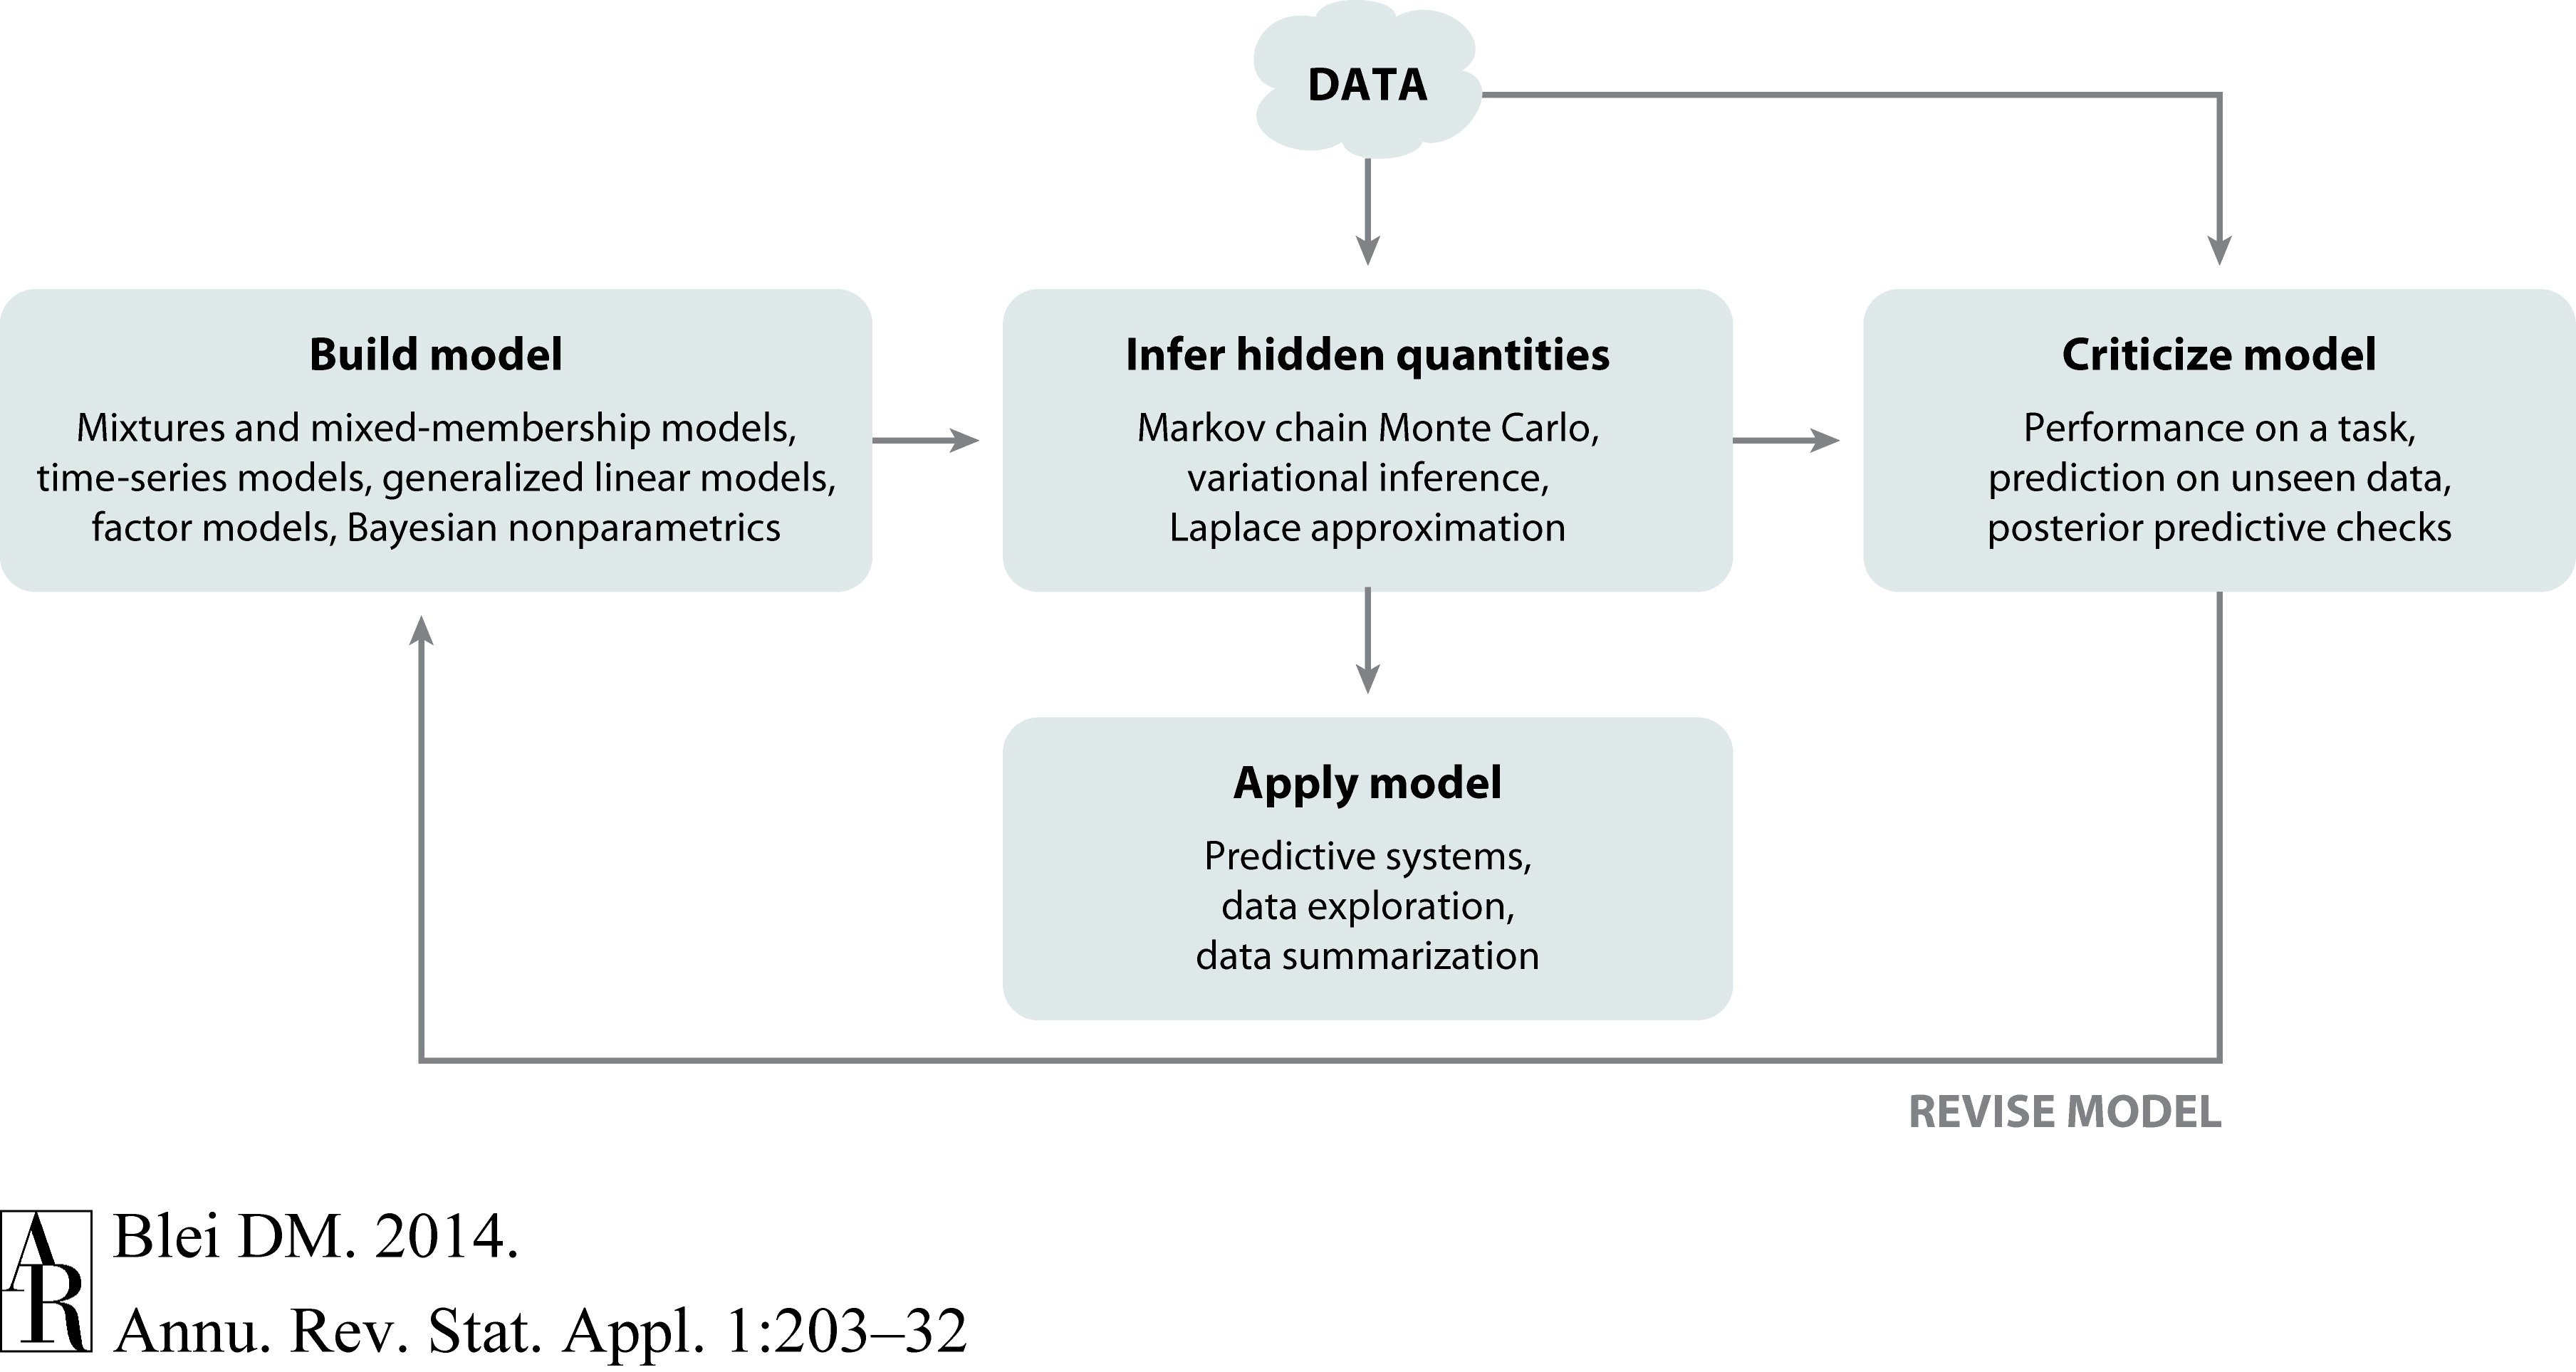
\includegraphics[width=.85\linewidth]{figures/lap1/boxsloop.jpeg}\\
\end{center} 
\begin{flushright}
{\footnotesize Blei, \textit{Ann. Rev. Stat. App.} 2014.}
\end{flushright}
\end{frame}

\begin{frame}{}
    \centering
    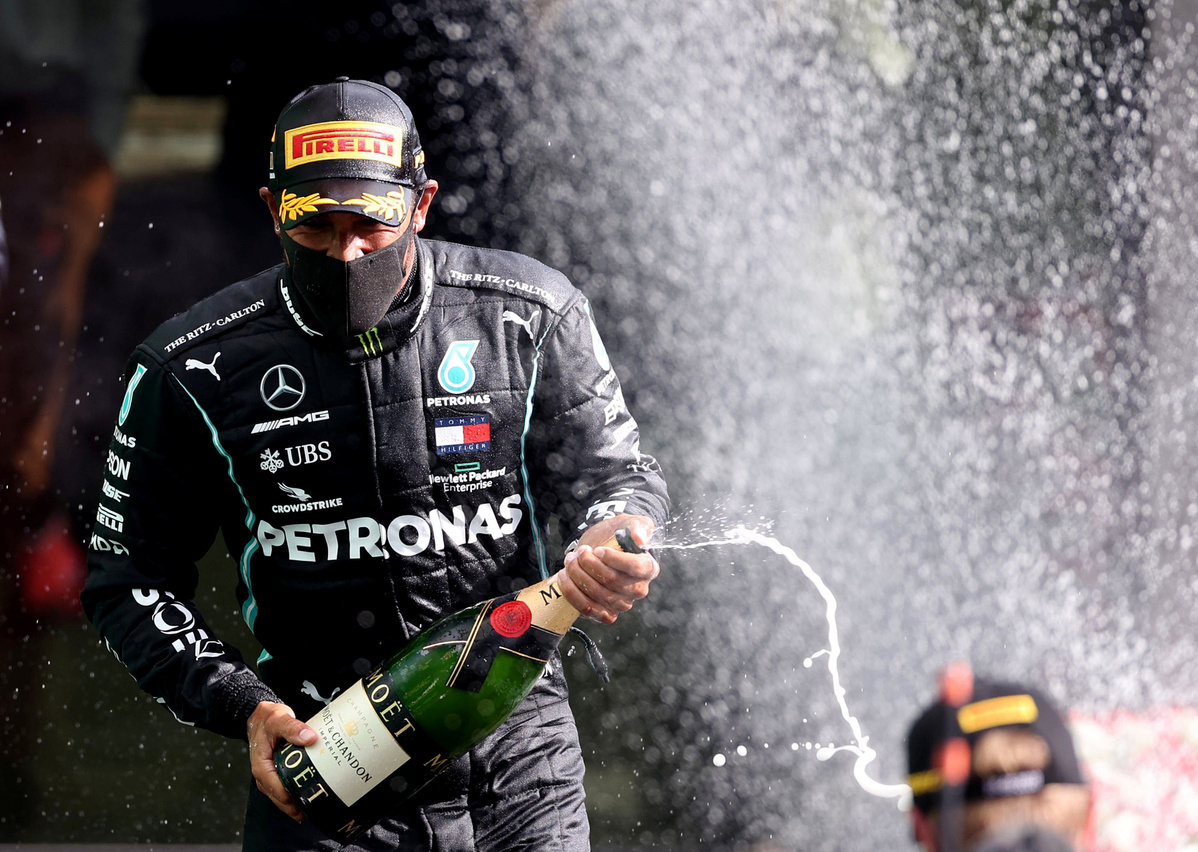
\includegraphics[width=.8\textwidth]{figures/lap9/hamilton.jpeg}
\end{frame}

\begin{frame}{Victory Lap: The great beyond}
\begin{itemize}
    \item Highlights
    \item Some things we missed
\end{itemize}
\end{frame}


\begin{frame}{Highlights}
    \begin{table}[]
        \centering
        \begin{tabular}{r|c|c|c}
                            &  \textbf{Model} & \textbf{Algorithm} & \textbf{Criticism}\\
             \hline 
             \textbf{Lap 1} &  Linear Regression & Exact Inference & Bayes Factors \\
             \textbf{Lap 2} &  Logistic Regression & Laplace Approx. & Predictive Likelihood \\
             \textbf{Lap 3} &  Robust Regression & MCMC / HMC & MCMC Diagnostics \\
             \textbf{Lap 4} &  Mixture Models & Gibbs Sampling & Posterior Predictive Checks \\
             \textbf{Lap 5} &  Mixed Membership Models & Coordinate Ascent VI & - \\
             \textbf{Lap 6} &  Factor Analysis \& VAEs & BBVI \& Amortization & - \\
             \textbf{Lap 7} &  State Space Models & Message Passing \& SMC & -\\
             \textbf{Lap 8} &  Gaussian Processes & Elliptical Slice Sampling & - \\
        \end{tabular}
        % \caption{Caption}
        \label{tab:highlights}
    \end{table}
\end{frame}

\begin{frame}{The road not taken}
\centering
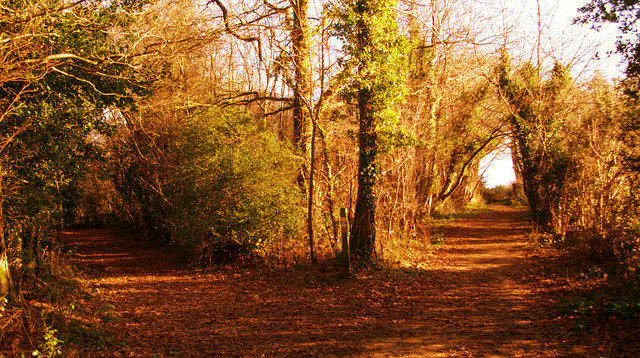
\includegraphics[width=.8\textwidth]{figures/lap9/road.jpeg}

\footnotesize \url{https://radiowest.kuer.org/}
\end{frame}

\begin{frame}{Hierarchical models}

Many datasets are organized into groups of observations, $\mbX = \{\{x_{g,n}\}_{n=1}^{N_g}\}_{g=1}^G$ where $G$ is the number of groups and $N_g$ is the number of observations in group $g$.

Two extreme models:
\begin{enumerate}
    \item All groups share the same parameters: 
    \begin{align}
        p(\mbX, \theta) &= p(\theta) \prod_{g=1}^G \prod_{n=1}^{N_g} p(x_{g,n} \mid \theta)
    \end{align}
    \item All groups have independent parameters:
    \begin{align}
        p(\mbX, \mbTheta) &= \prod_{g=1}^G p(\theta_g) \prod_{n=1}^{N_g} p(x_{g,n} \mid \theta_g)
    \end{align}
\end{enumerate}
Model 1 pools information across all data points when estimating $\theta$, but ignores variability between groups. Model 2 allows variability but shares no information.

\end{frame}

\begin{frame}{Hierarchical Models II}
Of course, there is a third way:
\begin{align}
    p(\mbX, \mbTheta) &= p(\theta_0) \prod_{g=1}^G p(\theta_g \mid \theta_0) \prod_{n=1}^{N_g} p(x_{g,n} \mid \theta_g)
\end{align}
Each group has its own parameters, but they are tied together via a hierarchical prior. Thus, we get the best of both worlds: parameter sharing and group-to-group variability.

A concrete example of \textbf{hierarchical Bayesian linear regression}:
\begin{multline}
    p(\{\{\mbx_{g,n}, y_{g,n}\}_{n=1}^{N_g}\}_{g=1}^G, \{\mbw_g, \sigma_g^2\}_{g=1}^G, \mbw_0)
    = \\
    \cN(\mbw_0 \mid \mbmu_0, \lambda_0^{-1} \mbI) \prod_{g=1}^G \bigg[ \cN(\mbw_g \mid \mbw_0, \lambda^{-1} \mbI)\,  \distInvChiSq(\sigma_g^2 \mid \nu, \tau^2) \prod_{n=1}^{N_g} \cN(y_{n,g} \mid \mbw_g^\top \mbx_n, \sigma_g^2) \bigg]
\end{multline}
\textbf{Questions: } What happens when $\lambda \to \infty$? What happens when $\lambda \to 0$? Same for $\lambda_0$. How could you share information about the variances, $\sigma_g^2$?
\end{frame}

\begin{frame}{Hierarchical Models III}
    Consider the question of determining $K$, the number of components in a mixture model.
    
    Rather than using predictive log likelihood to choose a single $K$ (recall Lap 4), we treat $K$ as a random variable in a hierarchical model,
    \begin{align}
        p(\{\mbx_n, z_n\}_{n=1}^N, \mbTheta, K) &= 
        p(K) p(\mbpi \mid K) \prod_{k=1}^K p(\theta_{k}) \prod_{n=1}^N p(z_n \mid \mbpi) \, p(\mbx_n \mid \theta_{z_n})
    \end{align}
    Suppose $K$ can take on a finite range of values in the set~$\cK$. The marginal distribution, summing over $K$, is a \textbf{mixture of finite mixture models}~\citep{Miller2018-dv}
    \begin{align}
        p(\{\mbx_n, z_n\}_{n=1}^N, \mbTheta) &= 
        \sum_{\kappa \in \cK} p(K=\kappa) \, p(\mbpi \mid \kappa) \prod_{k=1}^\kappa p(\theta_{k}) \prod_{n=1}^N p(z_n \mid \mbpi) \, p(\mbx_n \mid \theta_{z_n})
    \end{align}
    Note that the size of $\mbpi$ and the set $\{\theta_k\}_{k=1}^K$ changes with the random variable $K$. 
\end{frame}

\begin{frame}{Bayesian nonparametrics}
Taking this idea to its countably infinite limit $\cK = 1, 2, \ldots$, we arrive at Bayesian nonparametric mixture models. 

We discussed such a model---the Dirichlet process mixture model---in Lap 4, but that's one of many.

In fact, we've seen another Bayesian model already: Gaussian processes!

In general, BNP deals with priors on infinite dimensional objects; i.e. stochastic processes. 

Other examples include the beta process, which is useful for constructing nonparametric \textbf{factorial} latent variable models, and the Pitman-Yor process, which generalizes the DP to allow for power-law distributed weights.

\citet{orbanz2012lecture} is a great introduction to this research area. 

\end{frame}

\begin{frame}{Bayesian deep learning}
Gaussian processes gave us tools to reason about random functions. Not just point estimates; full posterior distributions. Of course, there's another cool function class in town---neural networks!

Recall the standard feedforward neural network from Lap 6. Each layer applies a linear function followed by an elementwise nonlinearity. 
\begin{align}
    \E[\mby_n \mid \mbx_n, \mbTheta] &= g(\mbW_L g(\mbW_{L-1} g(\ldots g(\mbW_1 \mbx_n +  \mbb_1) \ldots ) + \mbb_{L-1}) + \mbb_L)
\end{align}
where $\mbTheta = \{\mbW_\ell, \mbb_\ell\}_{\ell=1}^L$ is the set of weights and biases.

If we put a prior on the weights and biases, $p(\mbTheta)$, we have a random function $g: \reals^{D_x} \to \reals^{D_y}$. Both the prior on weights and the structure of the neural network determine the effective ``kernel,'' $\mathrm{Cov}(g(\mbx_n), g(\mbx_{n'}))$. 

Once again, \citet{neal1996bayesian} paved the way for this research area, deriving the ``neural network kernel'' for an infinitely wide single layer network with probit units.  

Several recent works have extended these techniques to other architectures~\citep{Garriga-Alonso2018-jx,De_G_Matthews2018-vo,Lee2017-sm,Yang2019-uu,Arora2019-uc}, including the \textbf{neural tangent kernel}~\citep{Jacot2018-dl}. See \cite{Wilson_undated-sv} for an introduction.

\end{frame}

\begin{frame}{Probabilistic programming}
Ultimately, this course has been about developing techniques for modeling generative processes as joint distributions over parameters, latent variables, and data. We introduced a series of algorithms for ``inverting'' the generative model to infer the latent states and parameters given data. 

However, those inference algorithms were often quite tailored to the model.

The past ten years have seen great advances in \textbf{probabilistic programming languages} like Stan, Church, Vatican, Anglican (sensing a trend?), Turing, Gen, Edward, Pyro, etc. These languages provide a way to specify the generative process (i.e. how to sample from the model), and then automate the inference algorithm. 

It's a compelling idea! There's still work to be done in order to design inference algorithms as effective as our handcrafted ones, but that gap is closing. 

\end{frame}

\begin{frame}{Automated model search}
    Probabilistic programming languages aim to automate inference. Is it possible to automate the model building process as well? In probabilistic programming parlance, is it possible to do program induction?
    
    It's an exciting idea! Much of science is about building an increasingly refined model of the world, and it advances with the creative sparks (what Popper called \textbf{``bold ideas, unjustified anticipations, and speculative thought''}) that cause us to revise our current models. Could a machine do that?
    
    The automated statistician (Lap 8) aims to do exactly that for the special case of Gaussian processes. Many other model search strategies have been put forward as well, but ultimately the combinatorial growth of the problem seems to necessitate something more intelligent than brute force or greedy approaches. 
    
    Exciting as it is, it's also somewhat sad... Box's loop of model building, inference, and criticism is what draws many of us to science and statistics in particular. As much as I love understanding, I also enjoy the pursuit.  
    
\end{frame}

\begin{frame}{Bayesian decision making}
Ultimately, what do we use models for?  Aside from understanding the universe and its complex generative processes, we use them to make decisions. 

Put differently, Box's loop often involves some \textbf{action} on the part of the scientist or policy maker. Those actions can incur some \textbf{loss} (or reward, if you like thinking positively), and they can yield new data to inform subsequent models. 

Bayesian decision theory involves averaging over uncertainty in latent variables and parameters to compute the expected loss of various decisions. 

Often, decisions are made sequentially, and your actions can influence the future state of the world and hence the available future actions and expected loss. This is where Bayesian decision theory meets \textbf{Markov decision processes, reinforcement learning, and control theory}.

One particular instance of such problems is \textbf{active learning}, aka \textbf{optimal experimental design}, where the goal is to infer model parameters using strategically chosen experiments. E.g. to learn the weights of a regression by querying chosen inputs $\mbx_n$. \textbf{Bayesian optimization}~\citep{shahriari2015taking} is one such example. 

\end{frame}

\begin{frame}[t]{Ask me anything}
What other topics are you interested in?
\end{frame}

\begin{frame}{Final logistics}
    
\begin{itemize}
    \item We'll have two poster sessions next week: \textbf{1pm Wednesday, June 2} and \textbf{1pm Thursday, June 3}.
    \item Please attend both if you can! Poster sessions are much more fun with an audience.
    \item Stay tuned for instructions on how to use GatherTown for the poster sessions.
    \item I am still planning to upload our solutions to the homework. They just need a bit of clean-up. 
    \item Please fill out the course feedback questionnaire! It will help us improve this course in the future.
\end{itemize}
\end{frame}

\begin{frame}{}
\centering
\Large \textbf{It's been a pleasure having all of you in class, virtually.\\ Thank you, and have a great summer!}


\includegraphics[width=.8\textwidth]{figures/lap9/summer.jpeg}
\end{frame}

\begin{frame}[t,allowframebreaks]
        \frametitle{References}
        \bibliographystyle{unsrtnat}
        \bibliography{refs.bib}
\end{frame}

\end{document}